\documentclass[conference,onecolumn]{IEEEtran}
\IEEEoverridecommandlockouts
% The preceding line is only needed to identify funding in the first footnote. If that is unneeded, please comment it out.
\usepackage{cite}
\usepackage{amsmath,amssymb,amsfonts}
\usepackage{algorithmic}
\usepackage{graphicx,subcaption}
\usepackage{float}
\usepackage{hyperref}
\usepackage{textcomp}
\usepackage{xcolor}
\usepackage{listings}
\usepackage{enumitem}
\usepackage{booktabs}
\usepackage{multirow}
\usepackage{array}
\usepackage{minted}

\DeclareMathOperator*{\argmax}{arg\,max}
\DeclareMathOperator*{\argmin}{arg\,min}

\def\BibTeX{{\rm B\kern-.05em{\sc i\kern-.025em b}\kern-.08em
    T\kern-.1667em\lower.7ex\hbox{E}\kern-.125emX}}

\IEEEoverridecommandlockouts

\lstset{
    language=MATLAB,             % Set language to MATLAB
    basicstyle=\ttfamily\small,  % Set font to small and monospaced
    keywordstyle=\color{blue},   % Color keywords
    stringstyle=\color{orange},   % Color strings
    commentstyle=\color{gray},   % Color comments
    showstringspaces=false,      % Do not display string spaces
    frame=single,                % Add a frame around the code
    breaklines=true              % Line breaks for long lines
}

\setlist[enumerate,1]{label=\arabic{enumi}.}
\setlist[enumerate,2]{label=(\alph*)}
\setlist[enumerate,3]{label=\roman*.}

\begin{document}

\title{\Large Assignment 5 --- Math Fundamentals for Robotics 16-811, Fall 2024}

\author{
      \IEEEauthorblockN{Mukai Yu}
      \IEEEauthorblockA{\textit{MSR, CMU} \\
            Pittsburgh, PA\\
            \href{mailto:mukaiy@andrew.cmu.edu}{mukaiy@andrew.cmu.edu}}
}

\maketitle

\begin{enumerate}
      \item Consider a plane curve $y(x)$ over the interval $[x_0, x_1]$, with specified endpoints $y_0 = y(x_0)$ and $y_1 = y(x_1)$.
            Assume that $y_0 > 0$ and $y_1 > 0$ and that $y(x) \geq 0$ for $x_0 \leq x \leq x_1$.
            Now imagine rotating the curve about the x-axis to obtain a surface of revolution.
            Find the $C^2$ curve $y(x)$ with specified endpoints that minimizes the surface area of this surface of revolution.

                  [Hint: This problem explores further some of the limitations of the Calculus of Variations.
                        Depending on the endpoint conditions there may or may not be a $C^2$ solution.
                        What does the optimal “curve” look like when it is not $C^2$?
                        Can you say how the endpoint conditions matter?
                        Be aware: There are many subtleties; don't expect to cover all, but explore what you can.]

      \item Using Calculus of Variations, show that the shortest curve between two points on a sphere is an arc of a great circle.
                  [Hints: There are different ways to solve this problem.
                        Here is one approach: Use spherical $(u, v)$ coordinates, where $x = R \sin v cos u, y = R \sin v \sin u, z = R \cos v,$ with $R$ the radius of the sphere.
                        (Do not worry about singularities in the representation.)
                        Rephrase 3D arclength $\sqrt{dx^2 + dy^2 + dz^2}$ as a function of $u, v, du, dv$.
                        View the curve as a function $v(u)$.
                        Observe that u does not appear directly in the resulting integrand for arclength, so replace the Euler-Lagrange equation with another, as in lecture.
                        You may find the following identity useful:
                        $$
                              \int \frac{a dw}{\sqrt{\sin^4 w - a^2 \sin^2 w}} = - \sin^{-1}(\frac{\cot w}{\sqrt{\frac{1}{a^2} - 1}}) + k,
                        $$
                        where a and k are appropriate constants.]

      \item In the brachistochrone problem (“ski-slope” in lecture), suppose the right endpoint $(x_1, y_1)$ is not specified exactly, but is merely constrained to satisfy an equation of the form $g(x, y) = 0$.
            Show that the optimizing curve $y(x)$ is perpendicular to the iso-contour $g(x, y) = 0$ at $(x_1, y_1)$.

                  [Hints: (i) Use an equation from lecture rather than derive everything from scratch.
                        (ii) Observe that the curves are written differently, one explicitly as $y(x)$, the other implicitly as $g(x, y) = 0$.
                        Think about how to compare the slopes of the two curves despite these different representations.]

      \item \begin{enumerate}
                  \item Using Lagrangian Dynamics, derive the relationship between joint torques and the angular state (angles, angular velocities, and angular accelerations) of the following balanced manipulator:
                        \begin{figure}[H]
                              \centering
                              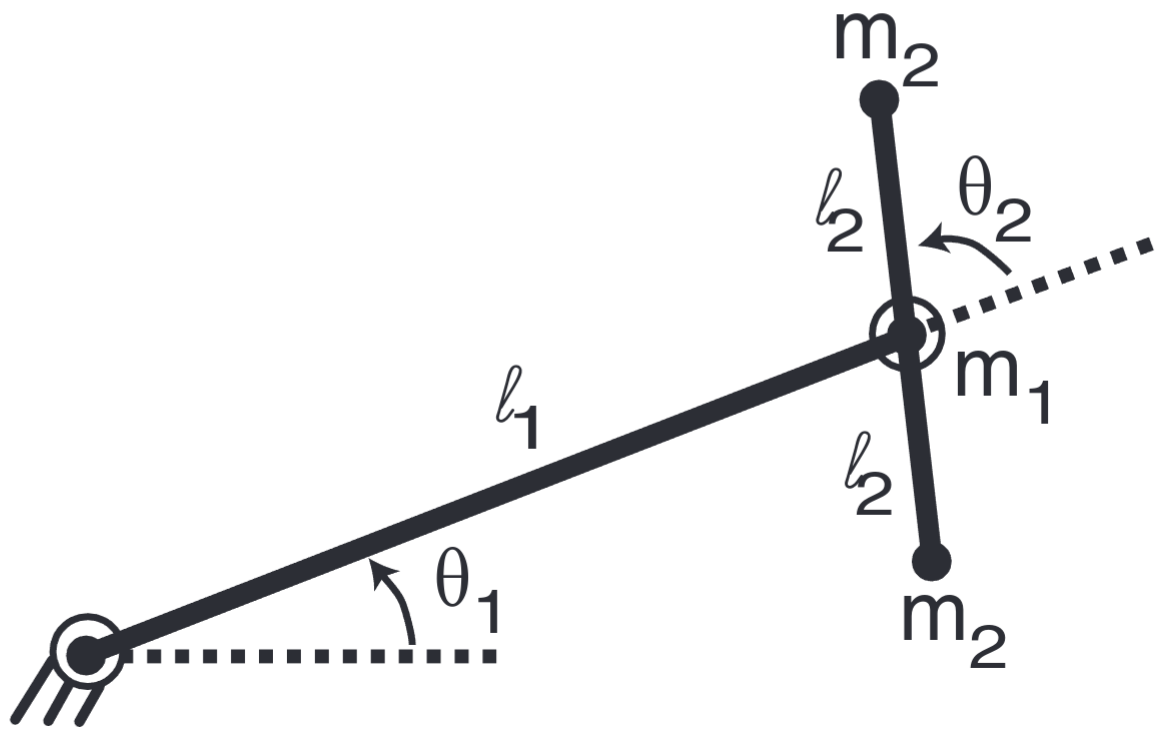
\includegraphics[width=0.5\linewidth]{figs/hw5_q4_fig1.png}
                        \end{figure}
                        There is no gravity (in practice, gravity is perpendicular to the sheet of the paper).

                        Legend: All of link \#1's mass, m1, is concentrated at distance $l_1$ from its rotational joint
                        (which is attached to the ground).
                        In turn, link \#2 rotates around this distal point, with two masses, $m_2$, located symmetrically, each at distance $l_2$, from the joint.
                        In practice, these two masses might constitute one counter-balanced end-effector or two different but equally weighted end-effectors.
                        — This is a variation of a basic SCARA-type robot arm, used in industrial assembly.
                  \item When $\ddot{\theta}_2 = 0$, explain the terms relating $\ddot{\theta}_1$ to $\tau_1$.
            \end{enumerate}
\end{enumerate}

\end{document}
